\documentclass[tikz,border=6pt]{standalone}
% Shared pastel academic grammar for final-size technical-paper diagrams.
\usepackage[T1]{fontenc}
\usepackage{lmodern}
\usepackage{amsmath,amssymb}
\usepackage{xcolor}
\usepackage{tikz}
\usetikzlibrary{
  arrows.meta,
  backgrounds,
  calc,
  circuits.logic.US,
  decorations.pathreplacing,
  fit,
  matrix,
  patterns,
  positioning,
  shapes.geometric,
  shapes.symbols
}

\definecolor{ink}{RGB}{24,24,28}
\definecolor{midink}{RGB}{96,96,104}
\definecolor{paleink}{RGB}{184,184,190}
\definecolor{wash}{RGB}{241,240,237}
\definecolor{paper}{RGB}{255,255,253}
\definecolor{cyan}{RGB}{126,203,218}
\definecolor{cyanwash}{RGB}{211,238,242}
\definecolor{pink}{RGB}{235,139,158}
\definecolor{pinkwash}{RGB}{250,211,217}
\definecolor{purple}{RGB}{166,50,150}
\definecolor{purplewash}{RGB}{232,196,227}
\definecolor{gold}{RGB}{177,139,45}
\definecolor{goldwash}{RGB}{239,226,183}
\definecolor{slate}{RGB}{116,133,145}
\definecolor{slatewash}{RGB}{221,226,229}
\colorlet{muted}{midink}
\colorlet{rule}{paleink}
\colorlet{accent}{purple}
\colorlet{accentwash}{purplewash}
\colorlet{second}{cyan}
\colorlet{secondwash}{cyanwash}

\tikzset{
  every picture/.style={
    font=\rmfamily\footnotesize,
    text=ink,
    line cap=round,
    line join=round,
    >=Stealth
  },
  every node/.style={outer sep=0pt},
  panel mark/.style={font=\rmfamily\bfseries\footnotesize},
  primary/.style={font=\rmfamily\footnotesize},
  secondary/.style={font=\rmfamily\scriptsize,text=midink},
  signal name/.style={font=\ttfamily\footnotesize,anchor=east},
  scope trace/.style={draw=ink,line width=.62pt,line cap=butt,line join=miter},
  hairline/.style={draw=paleink,line width=.28pt,line cap=butt},
  dotted guide/.style={draw=midink,line width=.32pt,densely dotted},
  dashed scope/.style={draw=ink,line width=.45pt,dashed},
  transition/.style={-{Stealth[length=1.8mm,width=1.25mm]},draw=ink,line width=.58pt},
  transition label/.style={font=\rmfamily\scriptsize,fill=paper,inner sep=1.2pt},
  preedge/.style={circle,draw=ink,fill=paper,line width=.58pt,minimum size=8.2mm,inner sep=1pt},
  observed preedge/.style={preedge,fill=purplewash,double,double distance=1.15pt,line width=.62pt,minimum size=9.8mm},
  brace/.style={decorate,decoration={brace,mirror,amplitude=3pt},draw=ink,line width=.45pt},
  grid rule/.style={draw=slate,line width=.32pt,line cap=butt},
  outer rule/.style={draw=ink,line width=.82pt,line cap=butt,line join=miter},
  star mark/.style={star,star points=5,star point ratio=2.2,draw=ink,fill=purple,minimum size=5.1mm,inner sep=0pt},
  % Compatibility vocabulary used by the repository's other figures.
  flow/.style={-{Latex[length=4.5pt,width=3.2pt]},draw=ink,line width=.55pt},
  heavy flow/.style={-{Latex[length=5pt,width=3.6pt]},draw=ink,line width=.8pt},
  wire/.style={draw=ink,line width=.5pt},
  bus/.style={draw=ink,line width=1.05pt},
  guide/.style={draw=midink,line width=.4pt,dotted},
  alternate/.style={draw=ink,line width=.5pt,dashed},
  scope/.style={draw=ink,line width=.5pt,dashed,inner sep=6pt},
  block/.style={draw=ink,line width=.55pt,fill=paper,minimum height=8mm,inner xsep=5pt,inner ysep=4pt,align=center},
  operation/.style={block,fill=cyanwash,minimum width=17mm},
  register/.style={block,fill=paper,minimum width=16mm,minimum height=10mm},
  state/.style={circle,draw=ink,line width=.55pt,fill=cyanwash,minimum size=8mm,inner sep=1pt,align=center},
  terminal/.style={state,fill=purplewash,double,double distance=1.2pt,line width=.6pt},
  predicate/.style={diamond,aspect=1.8,draw=ink,line width=.55pt,fill=pinkwash,inner xsep=3pt,inner ysep=2pt,align=center},
  datum/.style={rectangle,draw=ink,line width=.5pt,fill=goldwash,minimum width=8mm,minimum height=6mm,inner sep=2pt,align=center},
  panel label/.style={font=\rmfamily\bfseries\footnotesize},
  local heading/.style={font=\rmfamily\bfseries\footnotesize},
  annotation/.style={font=\rmfamily\scriptsize,text=midink,align=center},
  heading/.style={font=\rmfamily\bfseries\small},
  subheading/.style={font=\rmfamily\bfseries\footnotesize},
  note/.style={font=\rmfamily\scriptsize,text=midink},
  label/.style={font=\rmfamily\bfseries\scriptsize},
  mono/.style={font=\ttfamily\footnotesize},
  tiny mono/.style={font=\ttfamily\scriptsize},
  count/.style={font=\rmfamily\bfseries\small},
  selected/.style={draw=ink,fill=purplewash,line width=.8pt},
  cell on/.style={fill=purple,draw=ink,line width=.3pt},
  cell off/.style={fill=paper,draw=paleink,line width=.3pt}
}

% Flat pastel facets and depth edges for restrained axonometric constructions.
\tikzset{
  cyan facet/.style={draw=ink,fill=cyanwash,line width=.5pt,line join=round},
  cyan side/.style={draw=ink,fill=cyan,line width=.5pt,line join=round},
  pink facet/.style={draw=ink,fill=pinkwash,line width=.5pt,line join=round},
  pink side/.style={draw=ink,fill=pink,line width=.5pt,line join=round},
  purple facet/.style={draw=ink,fill=purplewash,line width=.55pt,line join=round},
  purple side/.style={draw=ink,fill=purple,line width=.55pt,line join=round},
  gold facet/.style={draw=ink,fill=goldwash,line width=.5pt,line join=round},
  gold side/.style={draw=ink,fill=gold,line width=.5pt,line join=round},
  context facet/.style={draw=ink,fill=slatewash,line width=.45pt,line join=round},
  depth edge/.style={draw=midink,line width=.38pt},
  surface grid/.style={draw=slate,line width=.32pt},
  projection/.style={draw=midink,line width=.38pt,densely dashed},
  accent curve/.style={draw=purple,line width=1.05pt},
  cyan curve/.style={draw=cyan!70!ink,line width=.9pt},
  pink curve/.style={draw=pink!70!ink,line width=.9pt},
  gold curve/.style={draw=gold!80!ink,line width=.9pt}
}


\tikzset{
  verdict state/.style={
    state,
    minimum size=13mm,
    font=\rmfamily\small,
    fill=paper,
    line width=.68pt
  },
  verdict before/.style={verdict state,fill=cyanwash},
  verdict first/.style={
    verdict state,
    fill=purplewash,
    double,
    double distance=1.05pt
  },
  verdict later/.style={verdict state,fill=pinkwash},
  tuple state/.style={
    state,
    minimum size=9.6mm,
    font=\ttfamily\footnotesize,
    fill=paper,
    line width=.58pt
  },
  tuple depth/.style={
    circle,
    draw=ink,
    fill=purplewash,
    line width=.35pt,
    minimum size=9.6mm,
    inner sep=1pt
  },
  tuple terminal/.style={
    tuple state,
    fill=purplewash,
    double,
    double distance=1.15pt,
    line width=.68pt
  },
  edge label/.style={
    font=\rmfamily\footnotesize,
    fill=paper,
    rounded corners=1pt,
    inner xsep=3pt,
    inner ysep=1.5pt,
    align=center
  },
  phase card/.style={
    draw=ink,
    fill=paper,
    line width=.45pt,
    rounded corners=2pt,
    minimum width=39mm,
    minimum height=15mm,
    font=\rmfamily\footnotesize,
    align=center,
    inner xsep=4pt,
    inner ysep=4pt
  },
  phase caption/.style={
    font=\rmfamily\itshape\scriptsize,
    text=midink,
    fill=paper,
    inner xsep=3pt
  },
  message label/.style={
    font=\rmfamily\scriptsize,
    align=center,
    fill=paper,
    fill opacity=.88,
    text opacity=1,
    rounded corners=1pt,
    inner xsep=2pt,
    inner ysep=1pt
  },
  message flow/.style={
    -{Stealth[length=1.8mm,width=1.25mm]},
    draw=ink,
    line width=.62pt,
    preaction={draw=purplewash,line width=2.35pt}
  },
  layer tag/.style={
    font=\rmfamily\bfseries\scriptsize,
    draw=ink,
    line width=.35pt,
    rounded corners=1.3pt,
    inner xsep=4pt,
    inner ysep=2pt
  }
}

% Keep the first four arguments machine-readable: index, x, y, physical tuple.
\newcommand{\messagestate}[6]{%
  \node[tuple state,#6] (m#1) at (#2,#3) {\texttt{#4}};
  \draw[guide] (m#1.south) -- ++(0,-.65mm);
  \node[message label,anchor=north] at ($(m#1.south)+(0,-.82mm)$)
    {$\mathrm{message}[#1]$\enspace #5};
}

\begin{document}
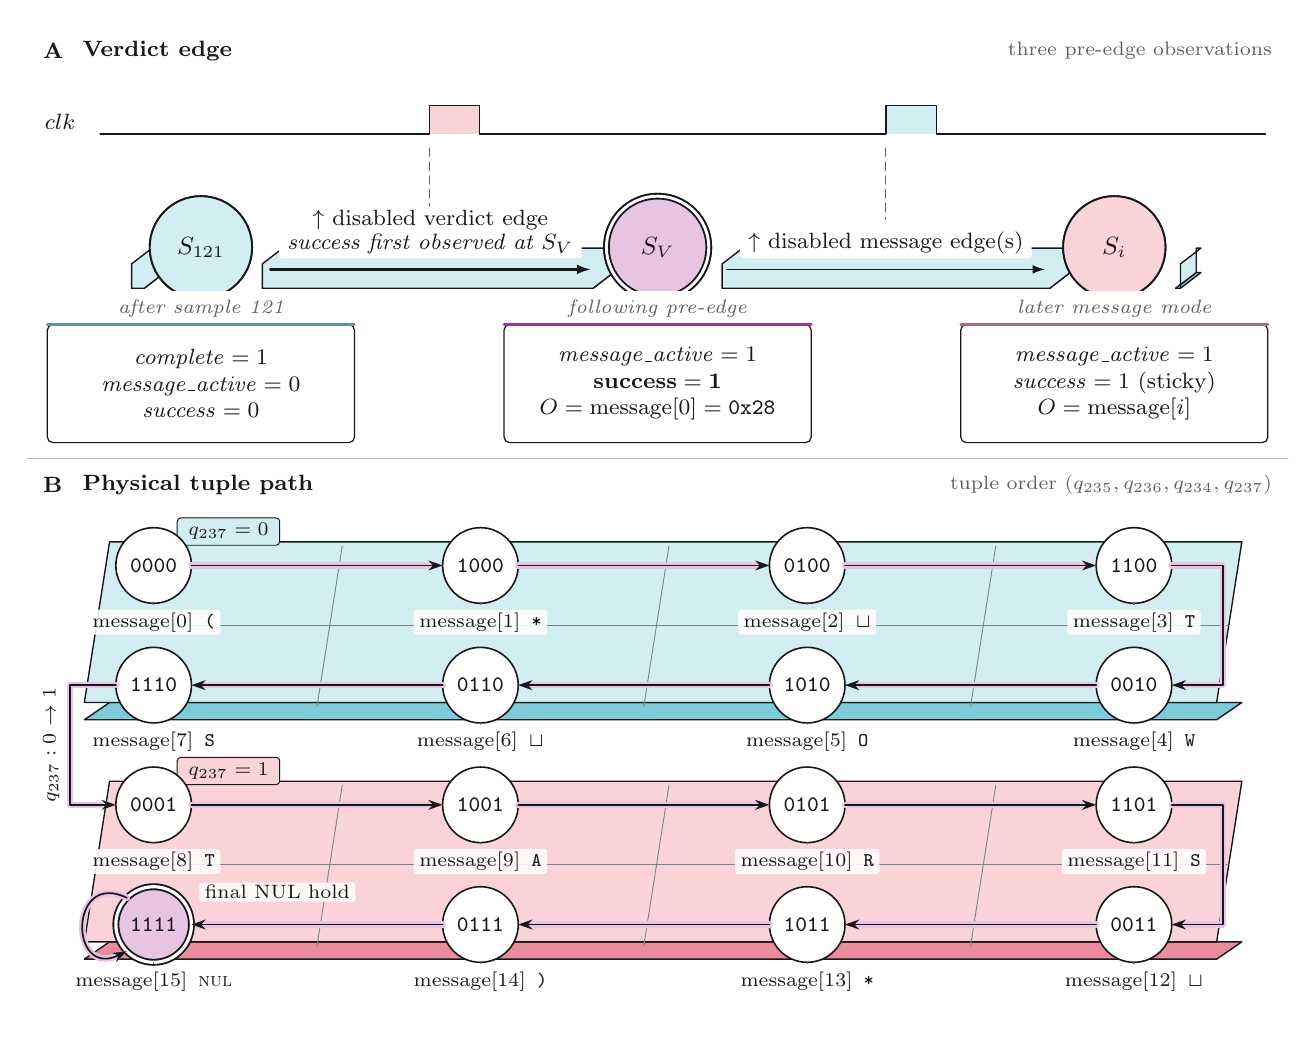
\begin{tikzpicture}[x=1cm,y=1cm]
  \path[use as bounding box] (0,0) rectangle (16,12.65);

  % A. Three exact pre-edge phases on a clock-aligned state ribbon.
  \node[panel label,anchor=west] at (.08,12.36) {A};
  \node[local heading,anchor=west] at (.58,12.36) {Verdict edge};
  \node[secondary,anchor=east] at (15.92,12.36)
    {three pre-edge observations};

  \node[font=\rmfamily\footnotesize,anchor=east] at (.72,11.46) {$clk$};
  \path[pink facet,draw=none] (5.10,11.30) rectangle (5.74,11.66);
  \path[cyan facet,draw=none] (10.90,11.30) rectangle (11.54,11.66);
  \draw[wire]
    (.92,11.30) -- (5.10,11.30) -- (5.10,11.66) --
    (5.74,11.66) -- (5.74,11.30) --
    (10.90,11.30) -- (10.90,11.66) --
    (11.54,11.66) -- (11.54,11.30) -- (15.72,11.30);
  \draw[projection] (5.10,11.12) -- (5.10,10.22);
  \draw[projection] (10.90,11.12) -- (10.90,10.22);

  % A shallow surface keeps the edge ordering visually continuous.
  \path[cyan side]
    (1.32,9.34) -- (1.48,9.34) -- (1.74,9.54) -- (1.58,9.54) -- cycle;
  \path[cyan facet,fill=cyanwash]
    (1.32,9.34) -- (1.48,9.34) -- (1.74,9.54) --
    (1.74,9.85) -- (1.58,9.85) -- (1.32,9.65) -- cycle;
  \path[cyan side]
    (2.98,9.34) -- (7.18,9.34) -- (7.44,9.54) -- (3.24,9.54) -- cycle;
  \path[cyan facet,fill=cyanwash]
    (2.98,9.34) -- (7.18,9.34) -- (7.44,9.54) --
    (7.44,9.85) -- (3.24,9.85) -- (2.98,9.65) -- cycle;
  \path[cyan side]
    (8.82,9.34) -- (12.98,9.34) -- (13.24,9.54) -- (9.08,9.54) -- cycle;
  \path[cyan facet,fill=cyanwash]
    (8.82,9.34) -- (12.98,9.34) -- (13.24,9.54) --
    (13.24,9.85) -- (9.08,9.85) -- (8.82,9.65) -- cycle;
  \path[cyan side]
    (14.64,9.34) -- (14.58,9.34) -- (14.84,9.54) -- (14.90,9.54) -- cycle;
  \path[cyan facet,fill=cyanwash]
    (14.64,9.34) -- (14.58,9.34) -- (14.84,9.54) --
    (14.84,9.85) -- (14.90,9.85) -- (14.64,9.65) -- cycle;

  \node[verdict before] (s121) at (2.20,9.86) {$S_{121}$};
  \node[verdict first] (sv) at (8.00,9.86) {$S_V$};
  \node[verdict later] (sm) at (13.80,9.86) {$S_i$};

  \draw[heavy flow] (3.08,9.58) --
    node[edge label,above=4pt]
      {$\uparrow$ disabled verdict edge\\[-.3mm]
       \textit{success first observed at $S_V$}}
    (7.15,9.58);
  \draw[flow] (8.88,9.58) --
    node[edge label,above=4pt]
      {$\uparrow$ disabled message edge(s)}
    (12.92,9.58);

  % Repaint the states after the edge arrows so the circles remain visually
  % intact on top of the ribbon and transition strokes.
  \node[verdict before] (s121) at (2.20,9.86) {$S_{121}$};
  \node[verdict first] (sv) at (8.00,9.86) {$S_V$};
  \node[verdict later] (sm) at (13.80,9.86) {$S_i$};

  \draw[projection] (s121.south) -- (2.20,9.08);
  \draw[projection] (sv.south) -- (8.00,9.08);
  \draw[projection] (sm.south) -- (13.80,9.08);

  \node[phase card] (card121) at (2.20,8.13)
    {$\mathit{complete}=1$\\
     $\mathit{message\_active}=0$\\
     $\mathit{success}=0$};
  \node[phase caption] at (2.20,9.08) {after sample 121};
  \draw[cyan curve] ([xshift=-19.5mm]card121.north) --
    ([xshift=19.5mm]card121.north);

  \node[phase card] (cardv) at (8.00,8.13)
    {$\mathit{message\_active}=1$\\
     $\mathbf{success=1}$\\
     $O=\mathrm{message}[0]=\mathtt{0x28}$};
  \node[phase caption] at (8.00,9.08) {following pre-edge};
  \draw[accent curve] ([xshift=-19.5mm]cardv.north) --
    ([xshift=19.5mm]cardv.north);

  \node[phase card] (cardm) at (13.80,8.13)
    {$\mathit{message\_active}=1$\\
     $\mathit{success}=1\ \text{(sticky)}$\\
     $O=\mathrm{message}[i]$};
  \node[phase caption] at (13.80,9.08) {later message mode};
  \draw[pink curve] ([xshift=-19.5mm]cardm.north) --
    ([xshift=19.5mm]cardm.north);

  \draw[rule,line width=.45pt] (0,7.18) -- (16,7.18);

  % B. Two ordered projection sheets, one for each q_237 layer.
  \node[panel label,anchor=west] at (.08,6.84) {B};
  \node[local heading,anchor=west] at (.58,6.84) {Physical tuple path};
  \node[secondary,anchor=east] at (15.92,6.84)
    {tuple order $(q_{235},q_{236},q_{234},q_{237})$};

  % Back sheet: q_237=0. The darker lower facet supplies restrained depth.
  \path[cyan side]
    (.72,3.86) -- (15.10,3.86) -- (15.42,4.08) -- (1.04,4.08) -- cycle;
  \path[cyan facet,fill=cyanwash]
    (.72,4.08) -- (15.10,4.08) -- (15.42,6.12) -- (1.04,6.12) -- cycle;
  \foreach \x in {3.675,7.825,11.975}{
    \draw[surface grid] (\x,4.03) -- ({\x+.32},6.07);
  }
  \draw[surface grid] (.88,5.06) -- (15.26,5.06);
  \node[layer tag,fill=cyanwash] at (2.55,6.25) {$q_{237}=0$};

  % Front sheet: q_237=1, projected in the same physical tuple order.
  \path[pink side]
    (.72,.82) -- (15.10,.82) -- (15.42,1.04) -- (1.04,1.04) -- cycle;
  \path[pink facet,fill=pinkwash]
    (.72,1.04) -- (15.10,1.04) -- (15.42,3.08) -- (1.04,3.08) -- cycle;
  \foreach \x in {3.675,7.825,11.975}{
    \draw[surface grid] (\x,.99) -- ({\x+.32},3.03);
  }
  \draw[surface grid] (.88,2.02) -- (15.26,2.02);
  \node[layer tag,fill=pinkwash] at (2.55,3.21) {$q_{237}=1$};

  % The first four arguments remain fixed for robust tuple extraction.
  \messagestate{0}{1.60}{5.82}{0000}{\texttt{(}}{}
  \messagestate{1}{5.75}{5.82}{1000}{\texttt{*}}{}
  \messagestate{2}{9.90}{5.82}{0100}{$\sqcup$}{}
  \messagestate{3}{14.05}{5.82}{1100}{\texttt{T}}{}

  \messagestate{4}{14.05}{4.30}{0010}{\texttt{W}}{}
  \messagestate{5}{9.90}{4.30}{1010}{\texttt{O}}{}
  \messagestate{6}{5.75}{4.30}{0110}{$\sqcup$}{}
  \messagestate{7}{1.60}{4.30}{1110}{\texttt{S}}{}

  \messagestate{8}{1.60}{2.78}{0001}{\texttt{T}}{}
  \messagestate{9}{5.75}{2.78}{1001}{\texttt{A}}{}
  \messagestate{10}{9.90}{2.78}{0101}{\texttt{R}}{}
  \messagestate{11}{14.05}{2.78}{1101}{\texttt{S}}{}

  \messagestate{12}{14.05}{1.26}{0011}{$\sqcup$}{}
  \messagestate{13}{9.90}{1.26}{1011}{\texttt{*}}{}
  \messagestate{14}{5.75}{1.26}{0111}{\texttt{)}}{}
  \messagestate{15}{1.60}{1.26}{1111}{\textsc{nul}}{tuple terminal}

  \foreach \a/\b in {0/1,1/2,2/3,4/5,5/6,6/7,8/9,9/10,10/11,12/13,13/14,14/15}{
    \draw[message flow] (m\a) -- (m\b);
  }
  \draw[message flow]
    (m3.east) -- (15.18,5.82) -- (15.18,4.30) -- (m4.east);
  \draw[message flow]
    (m7.west) -- (.54,4.30) -- (.54,2.78) -- (m8.west);
  \node[message label,rotate=90] at (.30,3.54) {$q_{237}:0\to1$};
  \draw[message flow]
    (m11.east) -- (15.18,2.78) -- (15.18,1.26) -- (m12.east);

  \draw[message flow]
    (m15.north west) .. controls +(-.74,.36) and +(-.74,-.36) ..
    (m15.south west);
  \node[message label,anchor=west] at (2.18,1.67) {final NUL hold};
\end{tikzpicture}
\end{document}
